\documentclass[12pt]{article}

\usepackage[portuguese]{babel}
\usepackage{graphicx}
\usepackage[section]{placeins}
\usepackage{float}
\usepackage{url}
\graphicspath{ {figures} }
\author{Rafael Begnini de Castilhos}
\title{Computação em nuvem e suas aplicações: uma pesquisa sobre o estado da arte}
\date{\today}

\begin{document}

\maketitle

\begin{abstract}
O presente artigo visa fomentar um debate sobre o estado da arte das aplicações da computação em nuvem, a fim de prover ao leitor o material necessário para compreender a importância da multidisciplinaridade entre as mais diversas áreas da computação. A metodologia utilizada para realizar a coleta foi dada por intermédio de pesquisas bibliográficas buscando materiais publicados nos últimos 3 anos em periódicos e congressos nacionais e internacionais.

\textbf{Palavras-chave:} Computação; Nuvem; Infraestrutura; Redes; Web-services; Servidor-Cliente; Segurança.

\end{abstract}

\section{Introdução}

\subsection{Motivação}

O crescimento gradativo no interesse na área de computação em nuvem traz consigo confusões quanto as reais aplicações e metodologia de desenvolvimento dessa tecnologia, sendo que as observações realizadas são disseminadas principalmente por publicações equivocadas em portais que induzem a breve leitura sobre determinado assunto, acarretando em desinformação. 

Outrossim, a computação em nuvem é uma solução tão abrangente que entrega tecnologia da informação como um serviço \cite{oliveira}. É notável que a expansão da indústria seja suportada pelo avanço das tecnologias em redes de computadores e mais recentemente pelas possibilidades de aplicabilidade da computação em nuvem.

Desta forma, é de extrema importância que a comunidade científica elabore publicações que tenham o fito de colaborar com a formação de uma melhor fonte de conhecimento para o público geral. Da mesma forma, é desejável que a expansão do mercado de tecnologia corrobore e provenha suporte no avanço e manutenibilidade das tecnologias em redes de computadores em nuvem.

\subsection{Justificativa}

Com o mundo cada vez mais virtualizado, a \emph{Cloud Computing} é considerada uma ferramenta importante para aumentar a produtividade \cite{loos}. Por isso os conceitos que serão abordados em seguida estão em alta no âmbito mundial. Pesquisas e avanços vem são desenvolvidos todos os dias, tanto em ambiente acadêmico, quanto institucional, propiciando elevado grau de maleabilidade sob o entendimento do leitor.

Desse modo, é essencial que sejam realizadas revisões com frequência, com o fito de manter-se atualizado e verificar qual o estado atual dessas pesquisas. Somente a partir de um processo de revisão desses é possível compreender o estado da arte.

\subsection{Objetivos}

\subsubsection{Gerais}
Esse artigo possui como objetivo geral introduzir conceitos para o melhor entendimento do conteúdo, debater as principais aplicações na indústria e apontar os avanços importantes nessa área.

\subsubsection{Específicos}
Os objetivos específicos se propõem à ingressar o leitor no assunto de computação em nuvem, descrever de forma resumida as possíveis técnicas e aplicações disponíveis e relacionar o estado da arte com situações práticas.

\subsection{Organização}

Este artigo está organizado da seguinte forma:
Na seção 2, conceitos básicos, temos uma breve introdução aos conceitos que serão necessários para o entendimento do trabalho, a definição e explicação de Computação em nuvem, Infraestrutura e Aplicações. Na seção 3, trabalhos correlatos estão outras obras relacionadas da área, a fim de explicar a importância das aplicações em nuvem. Na seção 4, aspectos relevantes, são ressaltados os pontos específicos que devem ser levados em consideração quando tratamos de aplicações voltadas ao escopo de computação em nuvem; Na seção 5, problemas existentes, é exemplificado as dificuldades, dores e desafios associados à esta área de pesquisa; Na seção 6, soluções possíveis, pretende-se apresentar soluções para os desafios citados na quinta seção.  Na seção 7, entramos a fundo no desenvolvimento da solução proposta por Westphall \emph{et al.} \cite{westphall}. Na seção 8 são apresentadas as conclusões retiradas a partir da análise da bibliografia e trabalhos futuros a serem realizados. Por fim, em referências bibliográficas estão listados todos os trabalhos e artigos utilizados como base para a elaboração deste artigo.

\section{Conceitos básicos}

\subsection{Computação em nuvem}

O termo computação em nuvem é relativamente recente, porém historicamente não há um inicio claro, e seu conceito inicial originou-se na década de 60, onde o cientista da computação John McCarthy afirmou que iria acontecer com a informática o mesmo que aconteceu com a eletricidade, ou seja, as pessoas não necessitariam ter seus próprios geradores de energia elétrica.

Em 2006 a \emph{Amazon} amadureceu o conceito da \emph{Elastic Computing Cloud} onde os usuários podem criar e configurar suas próprias máquinas virtuais. Logo após, em 2008, é lançado o \emph{Google App Engine} com intuito de rodas aplicações, hospedar sites e armazenar dados.

Computação em nuvem é definida pelo \emph{National Institute of Standards and Technology (NIST)} como um modelo para permitir acesso sob demanda onipresente e conveniente via rede a um \emph{pool} de recursos computacionais compartilhados, que podem ser configuráveis (rede, servidor, armazenamento, serviços) sendo rapidamente provisionados e lançados com o mínimo de esforço.

As cinco características fundamentais são: serviço fornecido sob demanda, acesso a rede pública, pool de recursos, rápida elasticidade e medição dos serviços.
\subsection{Infraestrutura}

As informações não são alocadas em uma única máquina como é feito em um servidor físico, por isso é disponibilizado um conjunto de máquinas que realizam o processamento dessas informações, reduzindo significativamente a carga de trabalho nos computadores locais, uma vez que não precisam mais executar as aplicações.

É imperioso destacar que devido a isso, a demanda por \emph{hardware} no lado do usuário cai, e o único fator que deve ser levado em consideração é se a máquina do usuário é capaz de rodar o \emph{software} que proporciona a interface do sistema. Nesse caso o funcionamento ocorre de forma que os recursos são entregues ao cliente e os mesmos não precisam saber como funciona esse mecanismo ou a localidade em que esses dados estão fisicamente.

É uma solução abrangente, que entrega Tecnologia da informação como um serviço. Baseada na internet, os recursos são configurados para trabalhar lado a lado, facilitando o uso dos recursos acumulativos do sistema, evitando designar \emph{hardware} específico para uma tarefa.

A infraestrutura pode ser visualizada como sendo composta pela camada física e camada de abstração. A física consiste em todo o \emph{hardware} necessário para prover todos os serviços, incluindo servidor, armazenamento e componentes de rede. A de abstração é o \emph{software} que roda sobre a camada física.

\subsection{Aplicações}

A acessibilidade para esses serviços, se dá por meio de inúmeras empresas, entre elas, as mais populares são \emph{Amazon Web Services}, \emph{Google Cloud Plataform}, \emph{Microsoft Azure} e \emph{IBM Cloud}, que fornecem um núcleo de funcionalidades genérico, onde cada uma possui características e especificações únicas.

As soluções de computação em nuvem, garantem agilidade e desempenho, permitindo crescimento de ferramentas de colaboração integrando-as entre vários setores e minimizando erros.

\section{Trabalhos correlatos}

A tabela a seguir contendo uma revisão bibliográfica sistêmica realizada em buscas no \emph{Scholar Google} nos mostra que há uma quantidade massiva de trabalhos realizados na área de \emph{Cloud Computing}, esse comportamento também se aplica quando utilizamos as duas palavras-chave.

A pesquisa aponta que existe um interesse mundial no assunto, sendo que a maioria dos trabalhos sendo escritos em inglês mas espalhados em países pelo mundo todo.

\begin{center}
    \begin{tabular}{ | c | c | }
    \hline
    Palavras-chave & Resultados \\ 
    \hline
    Cloud computing & 2,340,000 \\  
    \hline
    Cloud security & 1,880,000 \\
    \hline
    Cloud computing network & 1,590,000 \\
    \hline
    Cloud infrastructure & 1,360,000 \\
    \hline
    Cloud computing web services & 947,000 \\
    \hline
    \end{tabular}
\end{center}

\subsection{Approaches and Issues of Cloud Computing Technology: A Review \cite{pethi}}

O artigo de B. Pethiyagoda e B. Hettige tem como premissa analisar as abordagens e serviços tecnológicos fornecidos pela tecnologia de computação em nuvem e os problemas que enfrentamos.

Atualmente, três tipos populares de modelos de serviço de computação em nuvem estão sendo adotados com sucesso pela indústria. 

Plataforma como serviço (PaaS) dá aos usuários controle sobre o design do aplicativo, mas não dá a eles controle sobre a infraestrutura física. 

Infraestrutura como serviço (FaaS) provem ao consumidor escolher o sistema operacional, banco de dados e ambiente de desenvolvimento de aplicativos, o que dá ao consumidor maior controle sobre o \emph{hardware} em comparação com a plataforma como serviço, tendo a possibilidade de configurar os servidores com base em suas necessidades, o que geralmente inclui mais manutenção.

Software como serviço (SaaS) é um tipo de suporte a aplicativos baseado na Internet, na qual o usuário final não é obrigado a comprar ou manter o \emph{software}, pois é obtido do provedor de serviços que estão hospedados em uma infraestrutura em nuvem.

No entanto, uma série de questões prevalecem e precisam de atenção imediata. De acordo com os autores, os principais problemas são devido à segurança, performance e armazenagem dos dados.

\subsection{Pubic Cloud Computing: Big Three Vendors \cite{randa}}

O trabalho publicado por Alkhatib \emph{et al.} começa com uma conceituação em um escopo geral sobre as possibilidades providas pelos vendedores desses serviços.

São citadas e introduzidas os três principais agentes dessa proliferação de tecnologias, entre elas \emph{Amazon Web Services}, \emph{Google Cloud Plataform} e \emph{Microsoft Azure}.

Também fazem uma contextualização dos artifícios básicos que são utilizados por grande parte das aplicações. Por fim, é apresentado uma tabela de comparação dos recursos de cada um provedor, categorizando em \emph{Compute service}, \emph{Storage}, \emph{Database}, \emph{Backup}, \emph{Serverless computing}, \emph{Networking}, \emph{Security}, \emph{Location}, \emph{Documentation} e entre outros.

\subsection{A Comparative Analysis of Security Services in Major Cloud Service Providers \cite{guptha}}

No trabalho publicado por Guptha \emph{et al.} nós temos uma pesquisa de cunho prático, lidando diretamente com os serviços de segurança dos provedores observados (\emph{Amazon Web Services}, \emph{Google Cloud Plataform} e \emph{Microsoft Azure}). Segundo uma comparação entre os provedores, fica evidente que \emph{AWS} e \emph{Azure} possuem um número superior de serviços que ofertam variedades de funcionalidades referentes à segurança comparado com o \emph{Google Cloud}.

Além disso, de acordo com os autores, a \emph{Azure} é a opção mais barata, fornece mais melhor equilíbrio e maior variedade de conformidade
certificados e estruturas no comparativo entre as demais, 

O artigo conclui que \emph{AWS} e \emph{Azure} são o serviço de nuvem ideal provedores em termos apenas de recursos de segurança, número de serviços, popularidade e custo.

\subsection{Privacy and Security Issues in Cloud Computing: A Survey Paper\cite{bamasoud}}

Neste artigo, os autores revisam questões de segurança e privacidade, gargalos associados à nuvem computação e as questões específicas de segurança na computação em nuvem camadas e vulnerabilidades e como evitá-las e controlá-las.

Em específico, no ponto de vista do usuário, a computação em nuvem parece ser muito insegura devido a vulnerabilidades de segurança e falta de privacidade. 

Os pesquisadores apontam e detalham com precisão as possibilidades das existentes vulnerabilidades, entretanto, concluem que cabe aos desenvolvedores e engenheiros resolver questões de segurança e fornecer soluções mais confiáveis em diferentes tipos de arquiteturas para torná-la mais útil e disponível para o público.

\subsection{Efficient Computing Resource Sharing for Mobile Edge-Cloud Computing Networks\cite{zhang}}

Não é novidade que grande parte do tráfego de informações se dá por intermédio de dispositivos celulares, nesse contexto, os autores visam elaborar estruturas e arquiteturas de ponta a fim de otimizar o uso e melhorar a experiência dos usuários.

Zhang \emph{et al.} propõe uma estrutura eficiente para a computação movel e computação em nuvem com objetivo de compartilhar recursos de computação com uns aos outros para melhorar a lucratividade. Levando em consideração que a nuvem tem uma construção relativamente de baixo custo de operação devido ao recurso de construção centralizado e as economias em escala, entretanto o aumento exponencial de requisitos computacionais não trazem apenas um desafio, mas também aumenta o custo de operação intensamente.

Diante disso, os resultados da simulação mostram que a ferramenta proposta pode maximizar o lucro e promover o bem-estar social.

\subsection{Relação e Comparação com Trabalhos Correlatos}

Em comparação aos trabalhos correlatos descritos acima, este trabalho propõe uma arquitetura de monitoramento para nuvens privadas (PCMONS). Este trabalho também leva em consideração a privacidade e performance do ambiente em nuvem, seja em privadas ou públicas. Atrelado a esse panorama, é apresentado algumas possíveis soluções para cada cenário com problemas, chegando em uma conclusão e trabalhos futuros.

\section{Aspectos relevantes}
Após concluir a leitura dos artigos de base, foi constatado uma interdisciplinaridade expressiva referente à gama de contextos em que a computação em nuvem pode ser aplicada.

Preambularmente, por se tratar de uma área em ascensão, o espaço para novas e criativas ideias se mostra enorme. Em termos de interações, existem vários cenários possíveis, geralmente, um consumidor de nuvem pode solicitar uma nuvem serviço de um provedor de nuvem, diretamente ou por meio de uma nuvem corretora, sendo que o auditor conduz auditorias independentes \cite{donno}. Isso impacta no desenvolvimento de padrões e soluções gerais, pois quanto mais variáveis possíveis de serem aplicadas ao sistema, maior a complexidade exigida sobre a área de cobertura e suporte.

Outro aspecto importante é aos modelos de implantação disponíveis: Nuvem privada é de uso exclusivo da organização e clientes, sendo que a infraestrutura está estabelecida nas premissas da organização. Na Nuvem pública, os serviços são disponibilizadas para todos os seus clientes, sendo que a infraestrutura está estabelecida no prestador dos serviços. A Nuvem híbrida combina dois ou mais modelos, compartilhando setores com um conjunto de organizações ou empresas. Por fim, a Nuvem comunitária é hospedada em um terceiro agente, sendo um modelo mutuamente compartilhado por entidades como bancos, governos e sociedades comerciais. 

Nesse viés, atualmente existem três tipo populares de serviços na computação em nuvem, que estão sendo adotados pela indústria, eles são: Plataforma como Serviço, provém benefícios de maior agilidade nos negócios do que um método tradicional, de acordo com Pethiyagoda e Hettige a próxima geração está prevista para revolucionar o campo de desenvolvimento, tornando-o simples para não programadores. Infraestrutura como Serviço exige que os usuários finais implantem e operem os serviços de \emph{software}, de forma análoga de como fariam em seu próprio data center. O consumidor pode escolher o sistema operacional, banco de dados e ambiente de desenvolvimento de aplicativos, o que dá o maior controle do consumidor sobre o \emph{hardware} em comparação com Plataforma como Serviço. Por último, o Software como Serviço suporta aplicativos baseados na Internet, no qual o usuário pode acessá-lo por intermédio do navegador, não sendo necessário comprar ou manter o \emph{software}, pois o provedor cuidará de todos os serviços necessários para seus clientes, tais como manutenção, modificação e atualizações.

Portanto, algumas vantagens da computação em nuvem são: Produtividade, pois ajuda os provedores de nuvem a otimizar o dia-a-dia operações de forma eficiente, permitindo-lhes a liberdade operar sem a intervenção de obsoletos sistemas legados. Escalabilidade, devido ao fato de permitir que as organizações facilmente e aumentem / diminuam rapidamente seus requisitos de negócios. E por fim a Segurança, que, quando aplicada da maneira adequada é robusta na proteção de dados confidenciais, garantindo criptografia de ponta a ponta, utilizando recursos de segurança sofisticados, além disso, cabe destacar que os usuários também podem apagar dados remotamente de as máquinas infectadas no caso de alguma violação para evitar que caia nas mãos erradas\cite{rani}.

\section{Problemas existentes}
\cite{rani} Apresenta que a tecnologia de computação em nuvem é apreciada devido à sua amplitude e acessibilidade a qualquer hora e em qualquer lugar. No entanto, uma série de problemas prevalecem na computação em nuvem e precisam de atenção. Foi possível identificar durante a leitura dos trabalhos correlatos que existem problemas de certa forma estão interconectados. Nessa seção, esses problemas serão esmiuçados para futura análise e proposição de soluções.

Primeiramente, é imperioso destacar que a privacidade é uma questão importante para a computação em nuvem, tanto em termos de conformidade legal quanto de confiança do usuário \cite{thakur}. A vulnerabilidade pode ser dada por diferentes métodos: As \emph{APIs} costumam ser um problema de proteção, pois não fornecem apenas às empresas a autoridade, mas também autentica e permite acesso para personalizar a capacidade dos serviços em nuvem para atender demandas. Os ataques de negação de serviço, são lançados para determinar um ponto de apoio para posteriormente sequestrar dados confidenciais. Além disso, os \emph{malwares} são injetados com códigos maliciosos manipulados como parte do código ou serviço que opera dentro dos próprios servidores em nuvem, se tornando um grande suspeito à problema. Não bastando isso, ainda pode acontecer um caso mais raro, que é da perda de dados confidenciais, quando as empresas não estabelecem sistemas de recuperação e acontece alguma catástrofe na região em que o \emph{data center} está localizado, tornando assim uma questão que não pode ser recuperada, pois não existem cópias fisicamente em outro local.

Posteriormente, existe um problema mundial, o qual as pessoas enfrentarão futuramente, que está conectado às limitações de \emph{hardware}, não havendo mais espaço para armazenamento de dados. Isso se deve ao fato de que as empresas não conseguem acompanhar o crescimento da largura de banda. Os provedores de nuvem e consumidores devem considerar a ideia de tráfego e suas implicações no posicionamento em cada nível do sistema, com o fito de reduzir os custos, e, para contornar isso, uma opção é realizar o envio de conjuntos de dados, conhecidos como lotes.

Outro problema conhecido e explorado por diversos autores, é a performance, pode-se concluir que o atraso que uma nuvem apresenta não é realmente desagradável, sendo que os serviços estão utilizando uma infraestrutura inteligente, com a latência reduzida. Entretanto, conforme citado anteriormente, existe uma gama repleta de contextos em que a computação em nuvem pode ser aplicada, desse modo, de acordo com \cite{prasad}, o escopo das aplicações é limitado apenas para países com conectividade de telefone móvel, pois se não houver, não será possível estabelecer uma conexão. Outro ponto que deve ser considerado no contexto de aplicações voltadas para a agricultura é o custo dos \emph{smartphones}, sendo que existe uma parcela de fazendeiros que não são capazes de efetuar a aquisição ou pagamento de serviços de cobertura de rede 3G/4G/5G. Conforme \cite{reza}, a computação em nuvem ainda apresenta carência em avaliação de desempenho e medidas especiais são necessárias para este trabalho.

Dado isso, urge a elaboração de ações, soluções, pesquisas e testes com o objetivo de mitigar tais casos problemáticos.

\section{Soluções possíveis}
Por tratar-se de uma área ampla, com diversos problemas que não foram citados na seção anterior por terem menor relevância ou possuírem pouco material de pesquisa acessível.

O primeiro problema a ser solucionado é a vulnerabilidade em \emph{APIs}, sejam elas desenvolvidos pelos grandes provedores de nuvem com objetivo de prover acesso ao desenvolvedores ou sejam elas desenvolvidas por profissionais da área da computação e disponibilizadas para o mundo, possuem pontos críticos suscetíveis a falhas, oferecendo acessos indevidos à chaves privadas e permissões incoerentes. Para mitigar isso, cabe aos desenvolvedores utilizarem as melhores práticas de desenvolvimento nas abordagens que envolvem autenticação, sempre manter as dependências atualizadas em suas últimas versões e praticar a manutenção no código fonte. À vista disto, com objetivo de evitar perdas e apagões totais quando ocorrer catástrofes, uma medida recomendada é descentralizar as informações, criar instâncias em outras regiões fisicamente ou até mesmo distribuir as informações em outros provedores em regiões distintas.

Em segundo lugar, é necessário desbravar uma metodologia para separar os dados úteis dos indesejados, e, possivelmente, reciclar para que esses recursos de armazenamento possam ser utilizados novamente. Na opinião de Pethiyagoda e Hettige, os desenvolvedores devem concentrar suas ações em otimizar o armazenamento, em vez de criar novos dados, pois conforme menciona \cite{shanthi}, as estrategias de armazenamento em nuvem e os modelos de serviço ainda estão em estágios iniciais. Para contornar esse cenário nebuloso, a padronização e uso de melhores metodologias de balanceamento de carga devem ser abordados para enfrentar esse problema. Concomitantemente, existe o paradigma \emph{Edge computing}, presente na computação distribuída pois traz o poder computacional e o armazenamento para perto da fonte, assim melhorando o tempo re resposta média das aplicações (devido a redução da latência), e também redução do uso e consumo de banda.

Ao que se refere ao problema de performance, a abordagem do modelo \emph{Serverless} que é propagada como uma tecnologia disruptiva e tendenciosa, prometendo não necessário gastar o dinheiro e esforço para comprar e configurar servidores, acaba tendo problemas de desempenho e limitação, se tornando frágil no quesito performance, perante a exigência da indústria. Em contra-partida, no contexto de conectividade de telefone móvel, a implantação da rede 5G deve crescer rapidamente nos próximos anos, sendo capaz de melhorar significativamente a conexão oriunda dos dispositivos móveis com a nuvem, e assim consequentemente conectando mais dispositivos à rede, ampliando o leque de aplicações possíveis de serem provisionadas na nuvem. Outro ponto a ser destacado é que aumentar a potência e a velocidade do data center nem sempre será eficiente.

Contudo, podemos vislumbrar o modo pelo qual a execução de novos sistemas em nuvem prove a alavancagem de novas proposições. Todas essas questões levantam duvidas sobre a percepção das dificuldades. Dado isso, é possível perceber cada vez mais o cuidado necessário para identificar esses pontos críticos, na determinação dos objetivos e metas.

\section{Projeto e Desenvolvimento de uma Proposta}
\cite{westphall} Apresenta uma experiência com nuvem privada, discutindo o design e implementação (PCMONS) por intermédio de um caso de estudo para ajudar novos adotantes de computação em nuvem à realizar boas decisões na construção e monitoramento de sistemas, abordando uma arquitetura com apenas soluções de código aberto.

\subsection{Arquitetura}
Os pesquisadores aplicaram a arquitetura descrita para uma aplicação representada na figura 1, que demonstra os níveis das camadas. Na camada de Infraestrutura consiste em instalações de serviços essenciais como hardware e rede, interagindo com o sistema operacional, licenças, \emph{hipervisores} e entre outros. A camada de integração é composta por recursos heterogêneos, requisitando uma interface comum para o acesso. Uma situação típica é quando o usuário solicita uma instanciação de máquina virtual. Um cenário possível é a presença de múltiplas plataformas para computação em nuvem, como \emph{Eucalyptus} e \emph{OpenNebula}. Já a camada de visualização apresenta como o monitoramento por meio de interfaces, nesta camada pode implementar diferentes visões, de acordo com as necessidades da empresa.

\begin{figure}[H]
    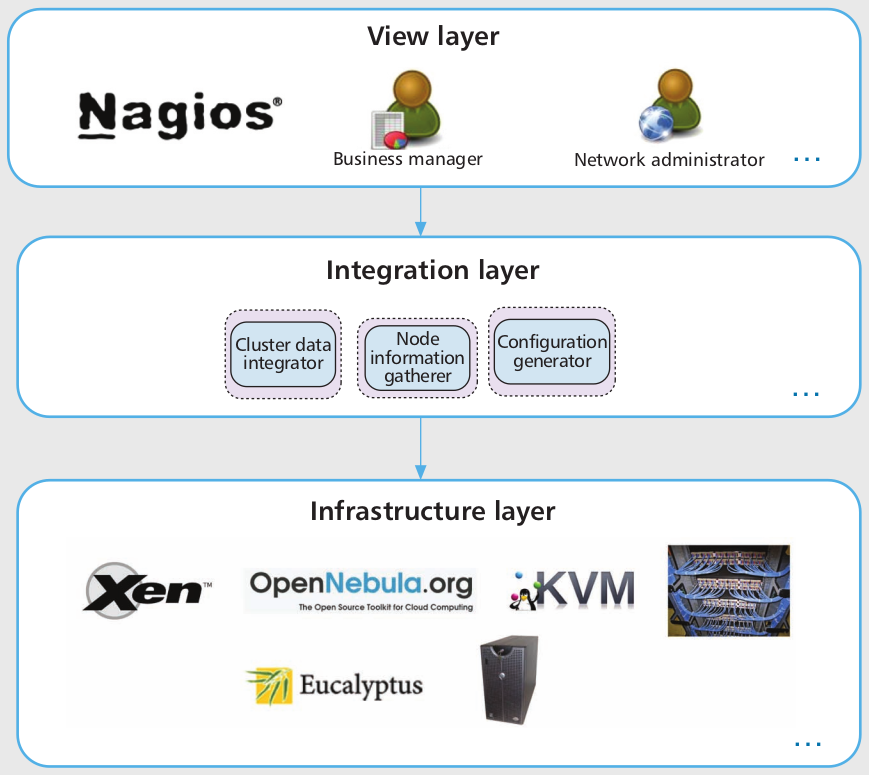
\includegraphics[width=\linewidth]{arquitetura.png}
    \caption{Arquitetura de sistema de monitoramento de nuvem privada.}
\end{figure}

\subsection{Caso de estudo}
Para concretizar o ambiente de teste apresentado na figura 2, o sistema operacional das máquinas físicas foi o \emph{SUSE} Linux, devido à sua fácil instalação e configuração. O \emph{Eucalyptus} é uma solução de software aberto para computação em nuvem que oferece uma interface compatível com \emph{Amazon EC2}. Para exemplificar a situação, foi construído um ambiente nas quais as maquinas virtuais estão disponíveis para usuários que instanciam um servidor web para hospedagem, utilizando ferramentas como \emph{Apache Web Server}, linguagem \emph{PHP} para desenvolvimento de páginas da Web e \emph{SQLite} para persistência de dados.

\begin{figure}[H]
    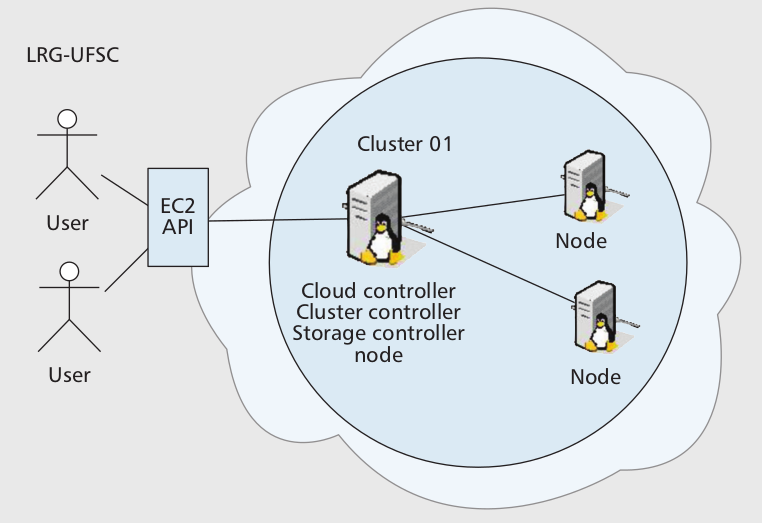
\includegraphics[width=\linewidth]{ambiente_teste.png}
    \caption{Um cenário de ambiente de teste.}
\end{figure}

Além das tecnologias destacadas acima, os autores utilizaram mais algumas, entre elas a linguagem \emph{Python} foi utilizada durante o desenvolvimento de processos, a linguagem \emph{Perl} também se fez necessário para realizar integrações com software \emph{Eucalyptus} e também a linguagem de \emph{script Bash} para realizar interações com Linux.

\subsection{Resultados obtidos}
A figura 3 mostra uma visão geral dos \emph{hosts} e grupos monitorados no estudo de caso. O \emph{Nagios} é utilizado para exibir as informações de monitoramento (colunas com nomes dos objetos, nomes dos serviços e seu respectivo status), permitindo possuir uma identificação ágil de falhas ou possíveis problemas durante a execução.

\begin{figure}[H]
    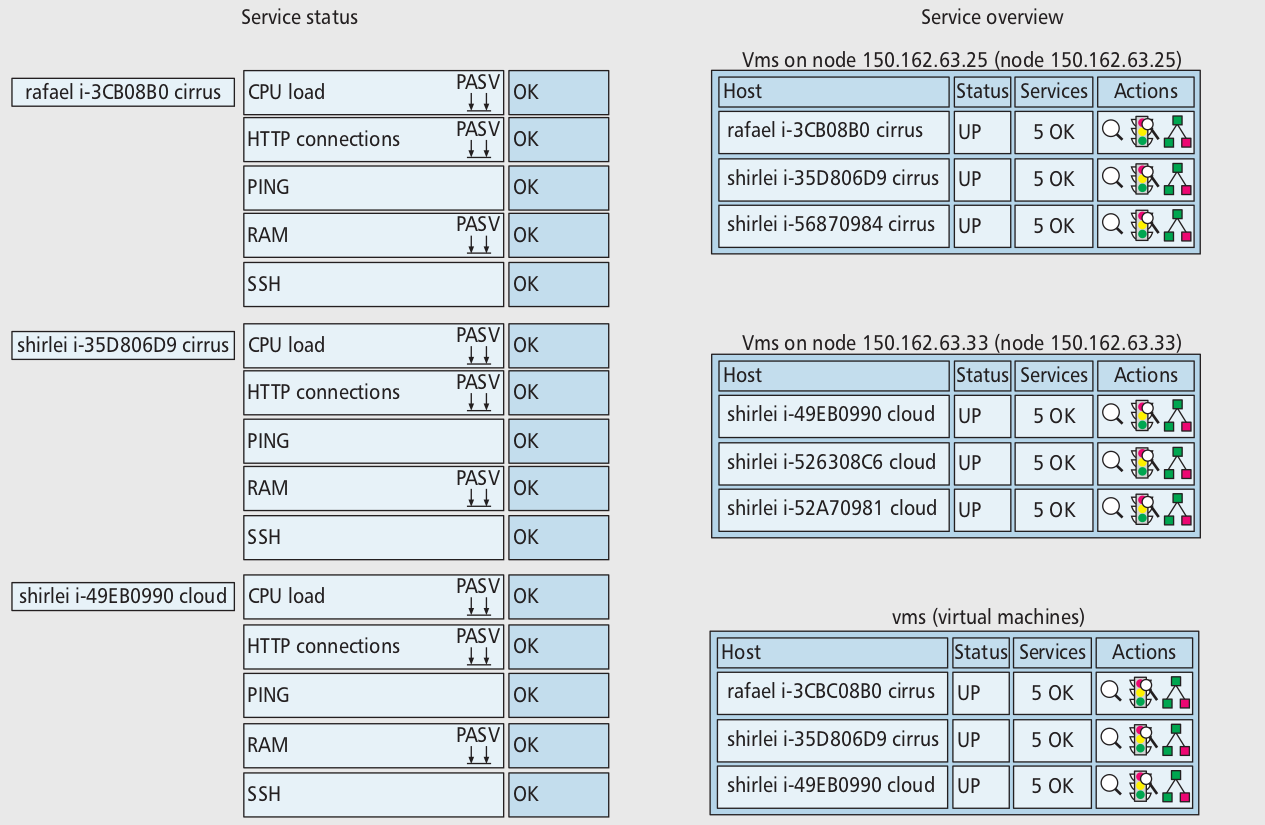
\includegraphics[width=\linewidth]{interface.png}
    \caption{Interface representativa do Nagios dos serviços de nuvem monitorados.}
\end{figure}

Durante o processo, os pesquisadores constataram que o monitoramento da computação em nuvem pode se beneficiar dos conceitos estabelecidos para computação distribuída. Em contrapartida, mesmo em nuvens privadas, a heterogeneidade dos recursos de computação pode exigir algum esforço extra ao implementar a solução de monitoramento. Por fim, a pesquisa fornece primeiros passos em direção a uma arquitetura de monitoramento para nuvens privadas. 

\section{Conclusões e Futuros Trabalhos}

\subsection{Conclusões}
Ao analisar uma pequena fração da ampla gama disponível de artigos e periódicos relacionados ao assunto estudado conseguimos obter um panorama do estado da arte, retirando conclusões que ainda podem ser remodeladas posteriormente.

Os problemas encontrados ao ler os materiais apontam para a necessidade do avanço e modernização da área de privacidade e performance, para aumentar e impulsionar a utilização dos recursos de computação em nuvem.

Fica evidente, que medidas precisam ser tomadas para atenuar os entraves destacados acima. Primeiramente, urge uma padronização das atuais plataformas de nuvem pelo menos de termos de interface, negociação e acesso através de serviços Web. Em paralelo, cabe às plataformas de nuvem não medirem esforços para promover o conhecimento, com propósito de ofertar o aprendizado na comunidade. Portanto, é expressivo o reconhecimento de pesquisas envolvendo computação em nuvem e suas aplicações somadas a arquitetura, como também a forma que o usuário cuida de sua infraestrutura e código, são essenciais nesse mundo a parte que está sendo criado pela computação.

\subsection{Futuros Trabalhos}
Como a tecnologia é crucial para as organizações, a computação em nuvem permite que as empresas sempre mantenham e acessem seus dados com segurança. Essa função resultou na crescente popularidade da computação em nuvem. Com o tempo, o serviço provedores se concentram em aumentar o número de serviços oferecidos, que incluem o aumento dos serviços analíticos. 

Estudos feitos pro \cite{randa}, comprovam a existência de uma competição muito acirrada pela liderança entre os três provedores de serviços em nuvem, ou seja, \emph{Amazon Web Services}, \emph{Google Cloud Platform} e \emph{Microsoft Azure}. Um ou mais modelos de entrega de computação em nuvem são suportado por cada um dos três grandes provedores de serviços em nuvem: \emph{PaaS, SaaS, DBaaS e IaaS}. A \emph{Amazon} é líder em \emph{IaaS}, enquanto o \emph{Google} se concentra mais na entrega de \emph{SaaS} e \emph{PaaS} modelos. A \emph{Microsoft} oferece essencialmente \emph{PaaS}, enquanto \emph{DBaaS} modelos são geralmente adotados pela \emph{Oracle, Amazon} e vários outros.

Ademais, para os trabalhos futuros, destaca-se a possibilidade de modelar e validar uma arquitetura genérica para aplicações que necessitam de um tempo de resposta excepcional, pesquisando sobre arquiteturas já existentes, identificando pontos fracos e fortes delas, a fim de construir um novo padrão capaz de se adaptar a uma boa gama de aplicações com pouca ou nenhuma modificação. A partir disso, é importante ressaltar a computação sem servidor (\emph{Serverless}) que é o serviço de nuvem estendida de mais rápido crescimento com um taxa de crescimento de 75 por cento, não sendo necessário gastar dinheiro e esforço para comprar e configurar servidores. 

\nocite{*}
\medskip

\bibliographystyle{unsrt}
\bibliography{biblio}

\end{document}